\section{Proprietà del getto}
Sulla base delle misure e dei profili di velocità media, effettuate al variare della distanza $x$ dalla sezione di uscita e del numero di Reynolds (portata del getto), si valutano gli andamenti di altre proprietà del getto una volta evidenziate le regioni caratteristiche nella precedente esercitazione.\\\\
In particolare, si vogliono valutare:
\begin{itemize}
    \item La velocità massima $U_{max}(x)$;
    \item La dimensione trasversale del getto $\Delta(x)$;
    \item La portata in massa $G(x)$;
    \item La quantità di moto $M(x)$;
    \item L'energia $E(x)$.
\end{itemize}
L'analisi dati per la presente attività è condotta con l'ausilio di un codice Python, riportato in appendice \ref{b4}.

\subsection{Velocità massima}
La velocità massima del getto per ogni profilo di velocità misurato risulta essere in prossimità dell'asse del getto. Si può quindi diagrammare l'andamento della velocità massima $U_{max}(x)$ in funzione della distanza assiale $x$.\\\\
Si evidenzia il noto risultato teorico per la velocità massima nella regione self-similare:
\begin{equation*}
    \frac{U_{max}(x)}{U_0} = \frac{k}{(x/D)^m}
\end{equation*}
Dove $k$ ed $m$ sono costanti da determinare sperimentalmente.\\\\
Rimaneggiando tale relazione, si ottiene:
\begin{equation*}
    \log \frac{U_{max}(x)}{U_0} = -m \log\frac{x}{D_j} + \log k
\end{equation*}
Imponendo le seguenti sostituzioni:
\begin{equation*}
    y = \log \frac{U_{max}(x)}{U_0} \qquad x = \log\frac{x}{D_j} \qquad q = \log k
\end{equation*}
Si evidenzia l'equazione di una retta:
\begin{equation*}
    y = -mx + q
\end{equation*}
Con una semplice interpolazione lineare dei dati nella regione autosimilare è dunque possibile ricavare i valori di $m$ e $k$ per le quattro squadre, si ottiene:
\begin{equation*}
    \begin{split}
        \text{Squadra 1: } m = 1.346 &\quad k = 8.377\\
        \text{Squadra 2: } m = 1.268 &\quad k = 8.368\\
        \text{Squadra 3: } m = 1.037 &\quad k = 7.110\\
        \text{Squadra 4: } m = 1.292 &\quad k = 12.781
    \end{split}
\end{equation*}
Utilizzando i valori di velocità massima per le quattro squadre, si ricava il seguente diagramma:
\begin{figure}[h]
    \centering
    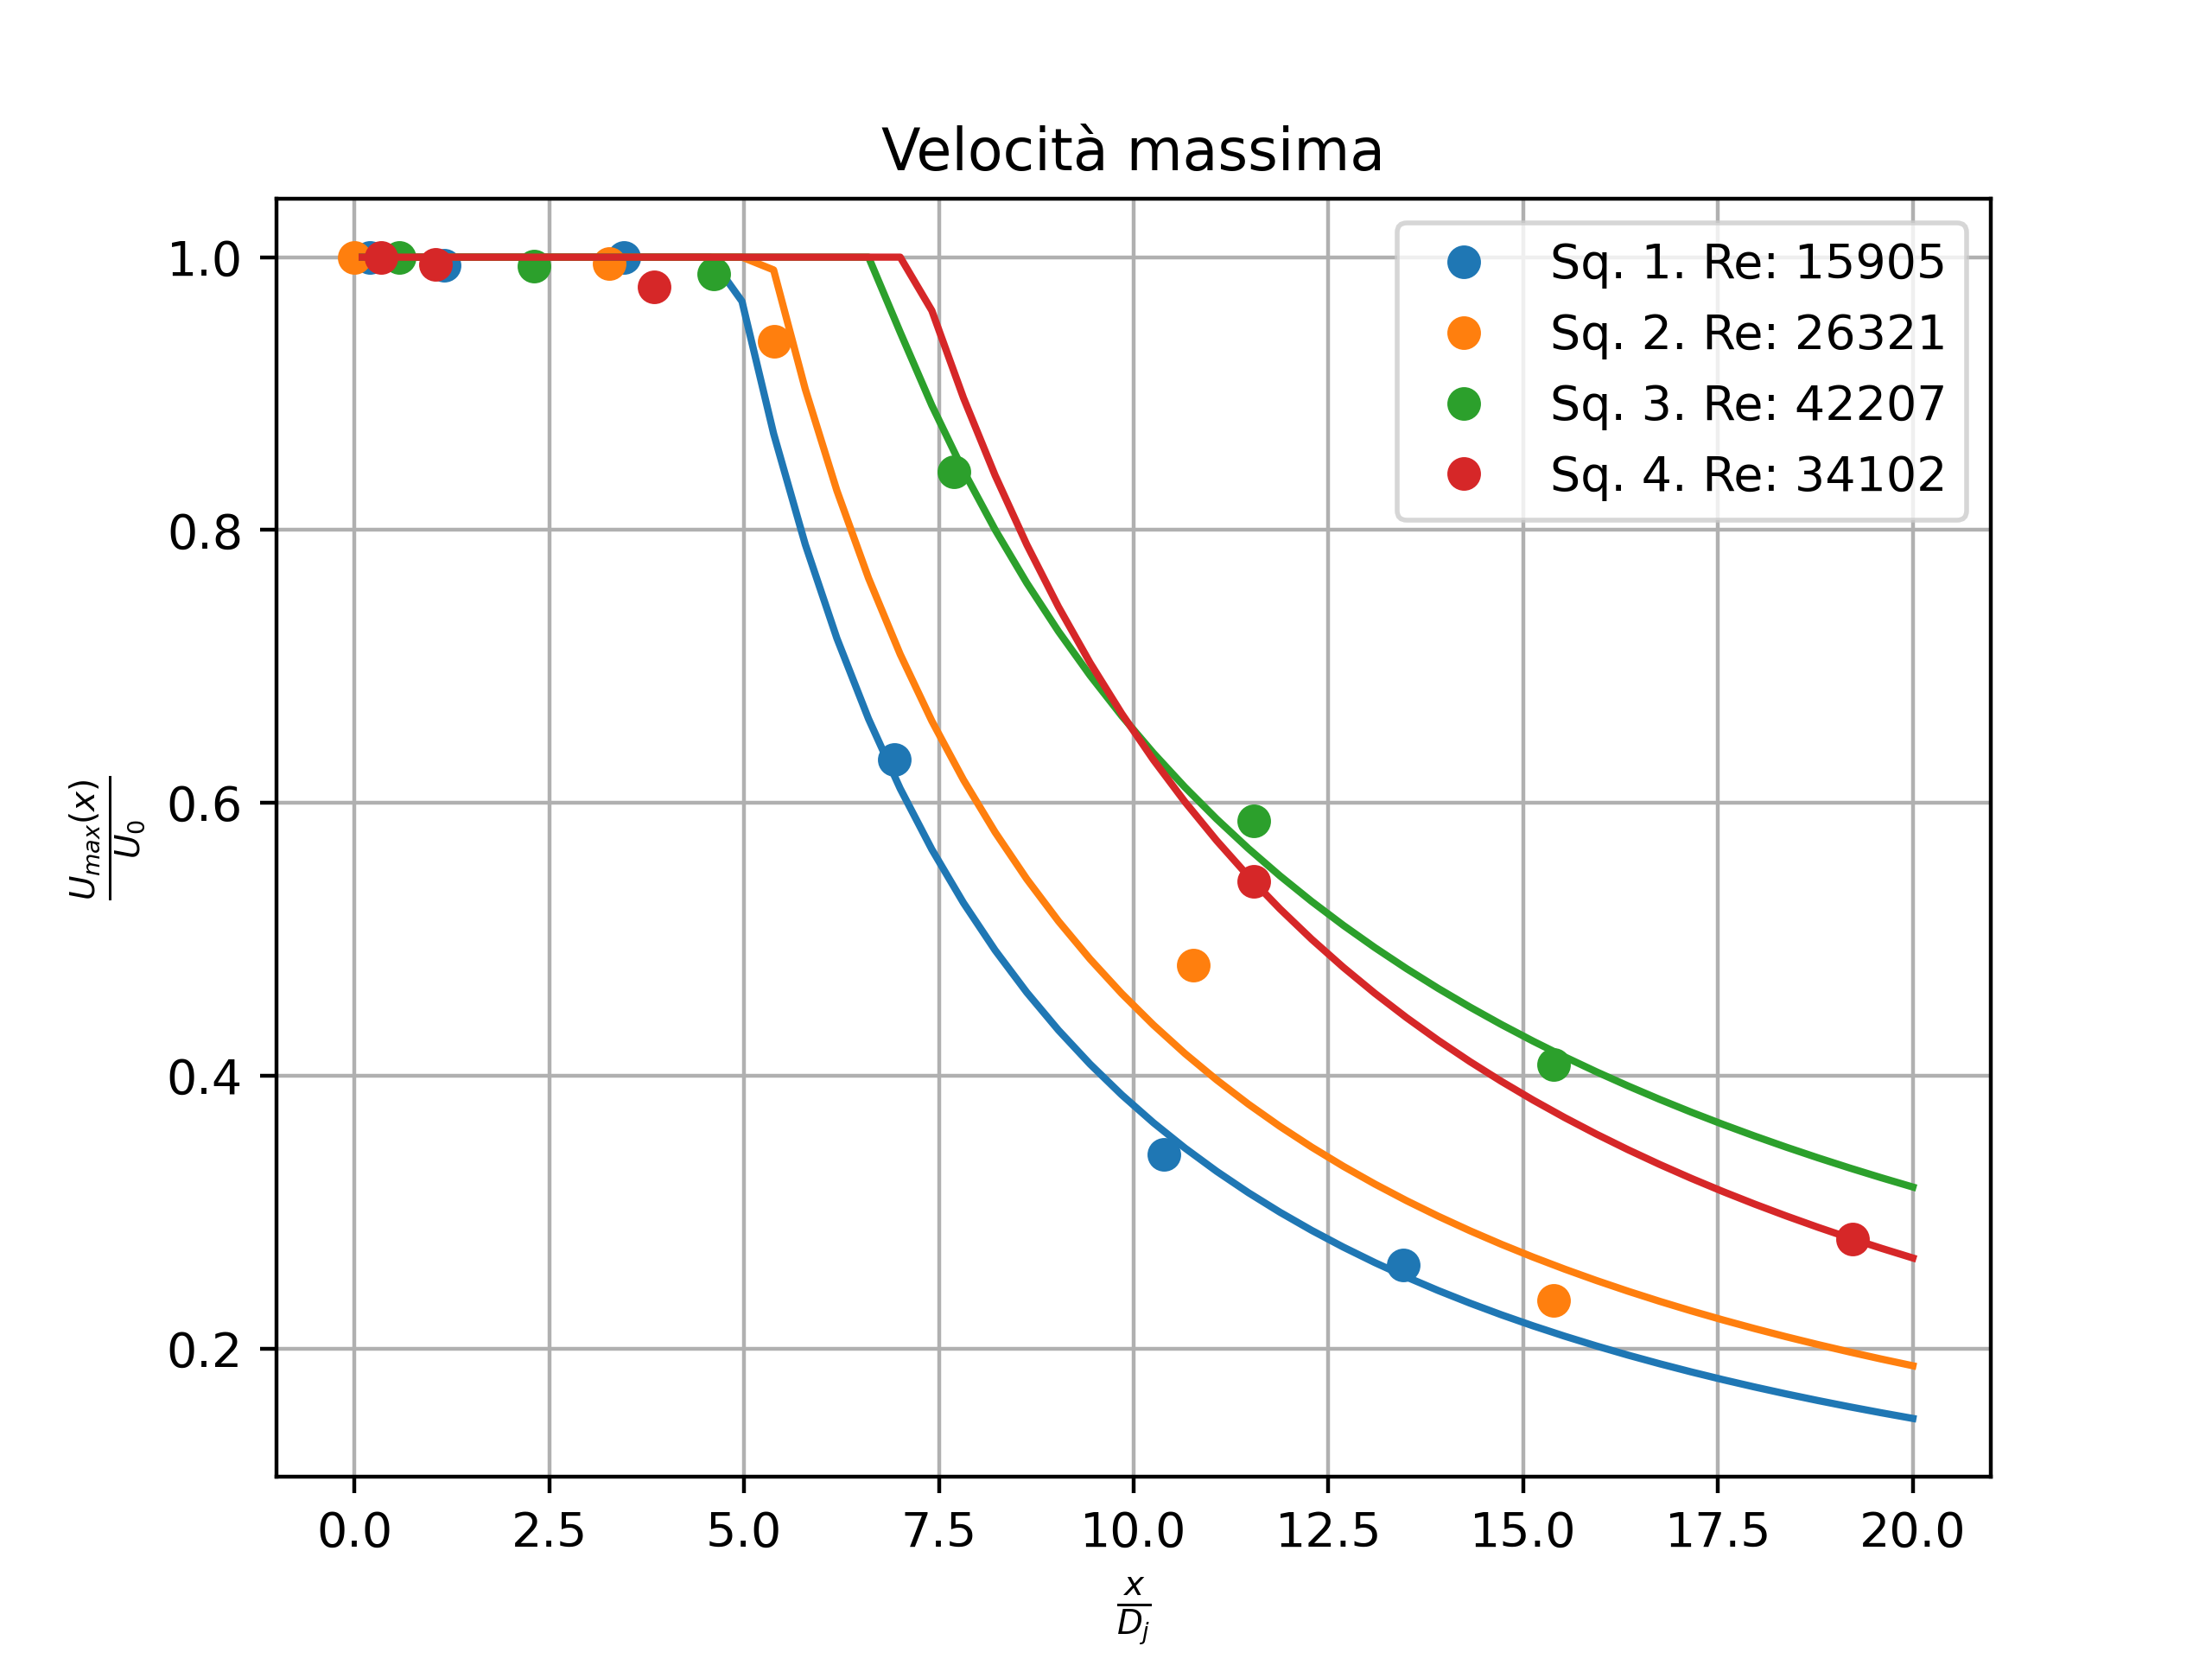
\includegraphics[width=.9\textwidth]{images/4/umax.png}
    \caption{Velocità massima lungo l'asse del getto}
\end{figure}

\noindent Il primo tratto costante evidenzia il cuore potenziale del getto, seguito dall'andamento esponenziale appena ricavato.\\\\
Si nota l'influenza del numero di Reynolds, infatti all'aumentare del numero di Reynolds aumenta la lunghezza assiale del cuore potenziale del getto, mentre nella regione self-similare per i quattro flussi analizzati la velocità massima decresce con un esponente $m$ che sembra non variare significativamente.

\subsection{Dimensione trasversale del getto}
Il getto trascina nel suo moto una quantità sempre crescente di fluido esterno a causa degli effetti viscosi (entrainment), quindi aumenta di spessore lungo l'asse.\\\\
La dimensione trasversale del getto è arbitrariamente definita come il valore di $r$ tale per cui la velocità è pari alla metà della velocità massima locale:
\begin{equation*}
    \Delta (x) = r_{U=0.5U_{max}(x)}
\end{equation*}
Si ottiene il seguente diagramma per le quattro squadre:
\begin{figure}[H]
    \centering
    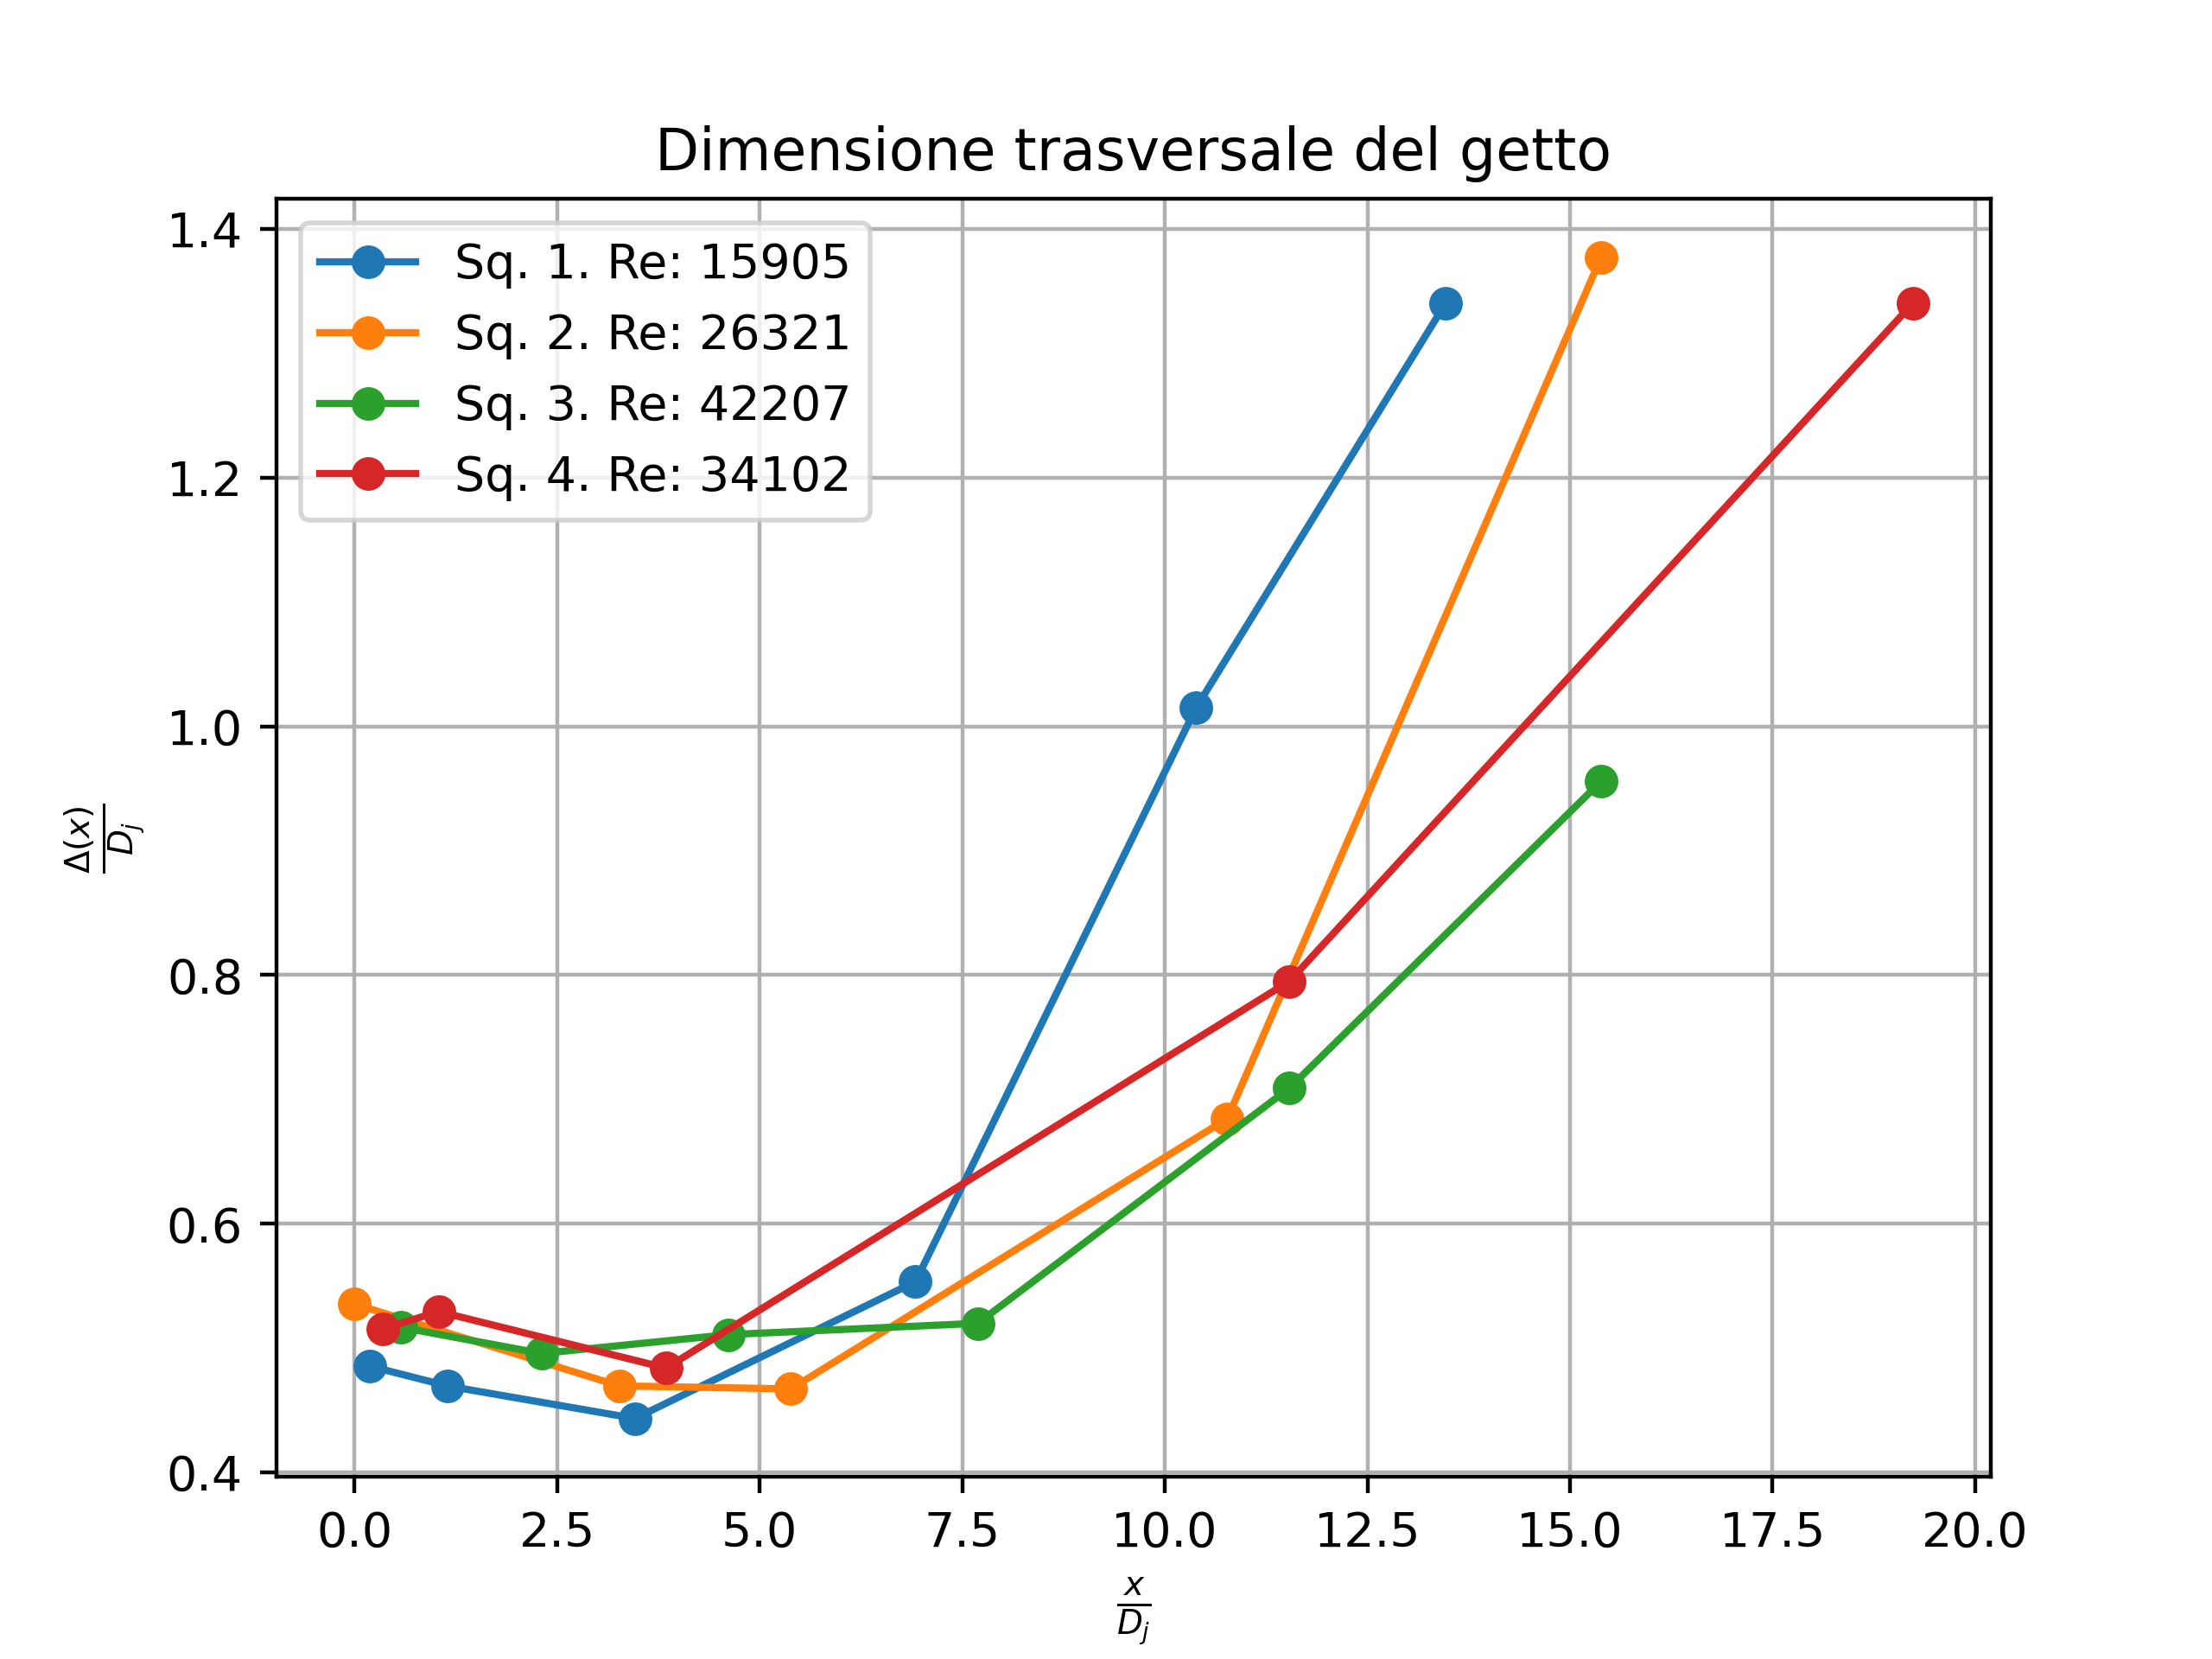
\includegraphics[width=.7\textwidth]{images/4/delta.png}
    \caption{Dimensione trasversale del getto}
\end{figure}
\begin{figure}[H]
    \centering
    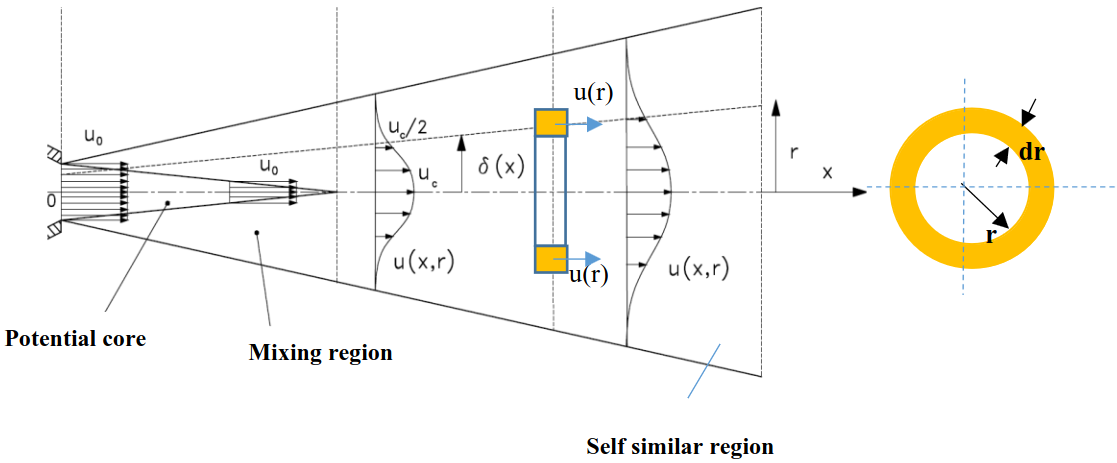
\includegraphics[width=.8\linewidth]{images/4/getto.png}
    \caption{Rappresentazione del getto}
\end{figure}

\subsection{Portata in massa}
A causa del trascinamento (entrainment) operato sul confine esterno del getto è atteso un aumento della portata in massa nella direzione dell'asse.\\\\
La portata elementare è definita come:
\begin{equation*}
    dG = \rho\ u\ dA = \rho\ u\ 2\pi rdr
\end{equation*}
Integrando si ottiene:
\begin{equation*}
    G = 2\pi\rho \int_0^\infty ur dr \quad \left[\frac{kg}{s} \right]
\end{equation*}
La portata in massa in corrispondenza della sezione di uscita è invece:
\begin{equation*}
    G_0 = \rho \left( \frac{\pi D^2}4 \right) U_0
\end{equation*}
Valutando la funzione integranda in modo discreto utilizzando i dati sperimentali, è possibile risolvere l'integrale con l'applicazione della regola dei trapezi.\\\\
Diagrammando l'andamento della portata $G$, normalizzata rispetto alla portata in corrispondenza della sezione di uscita $G_0$, si ottiene il seguente diagramma:
\begin{figure}[h]
    \centering
    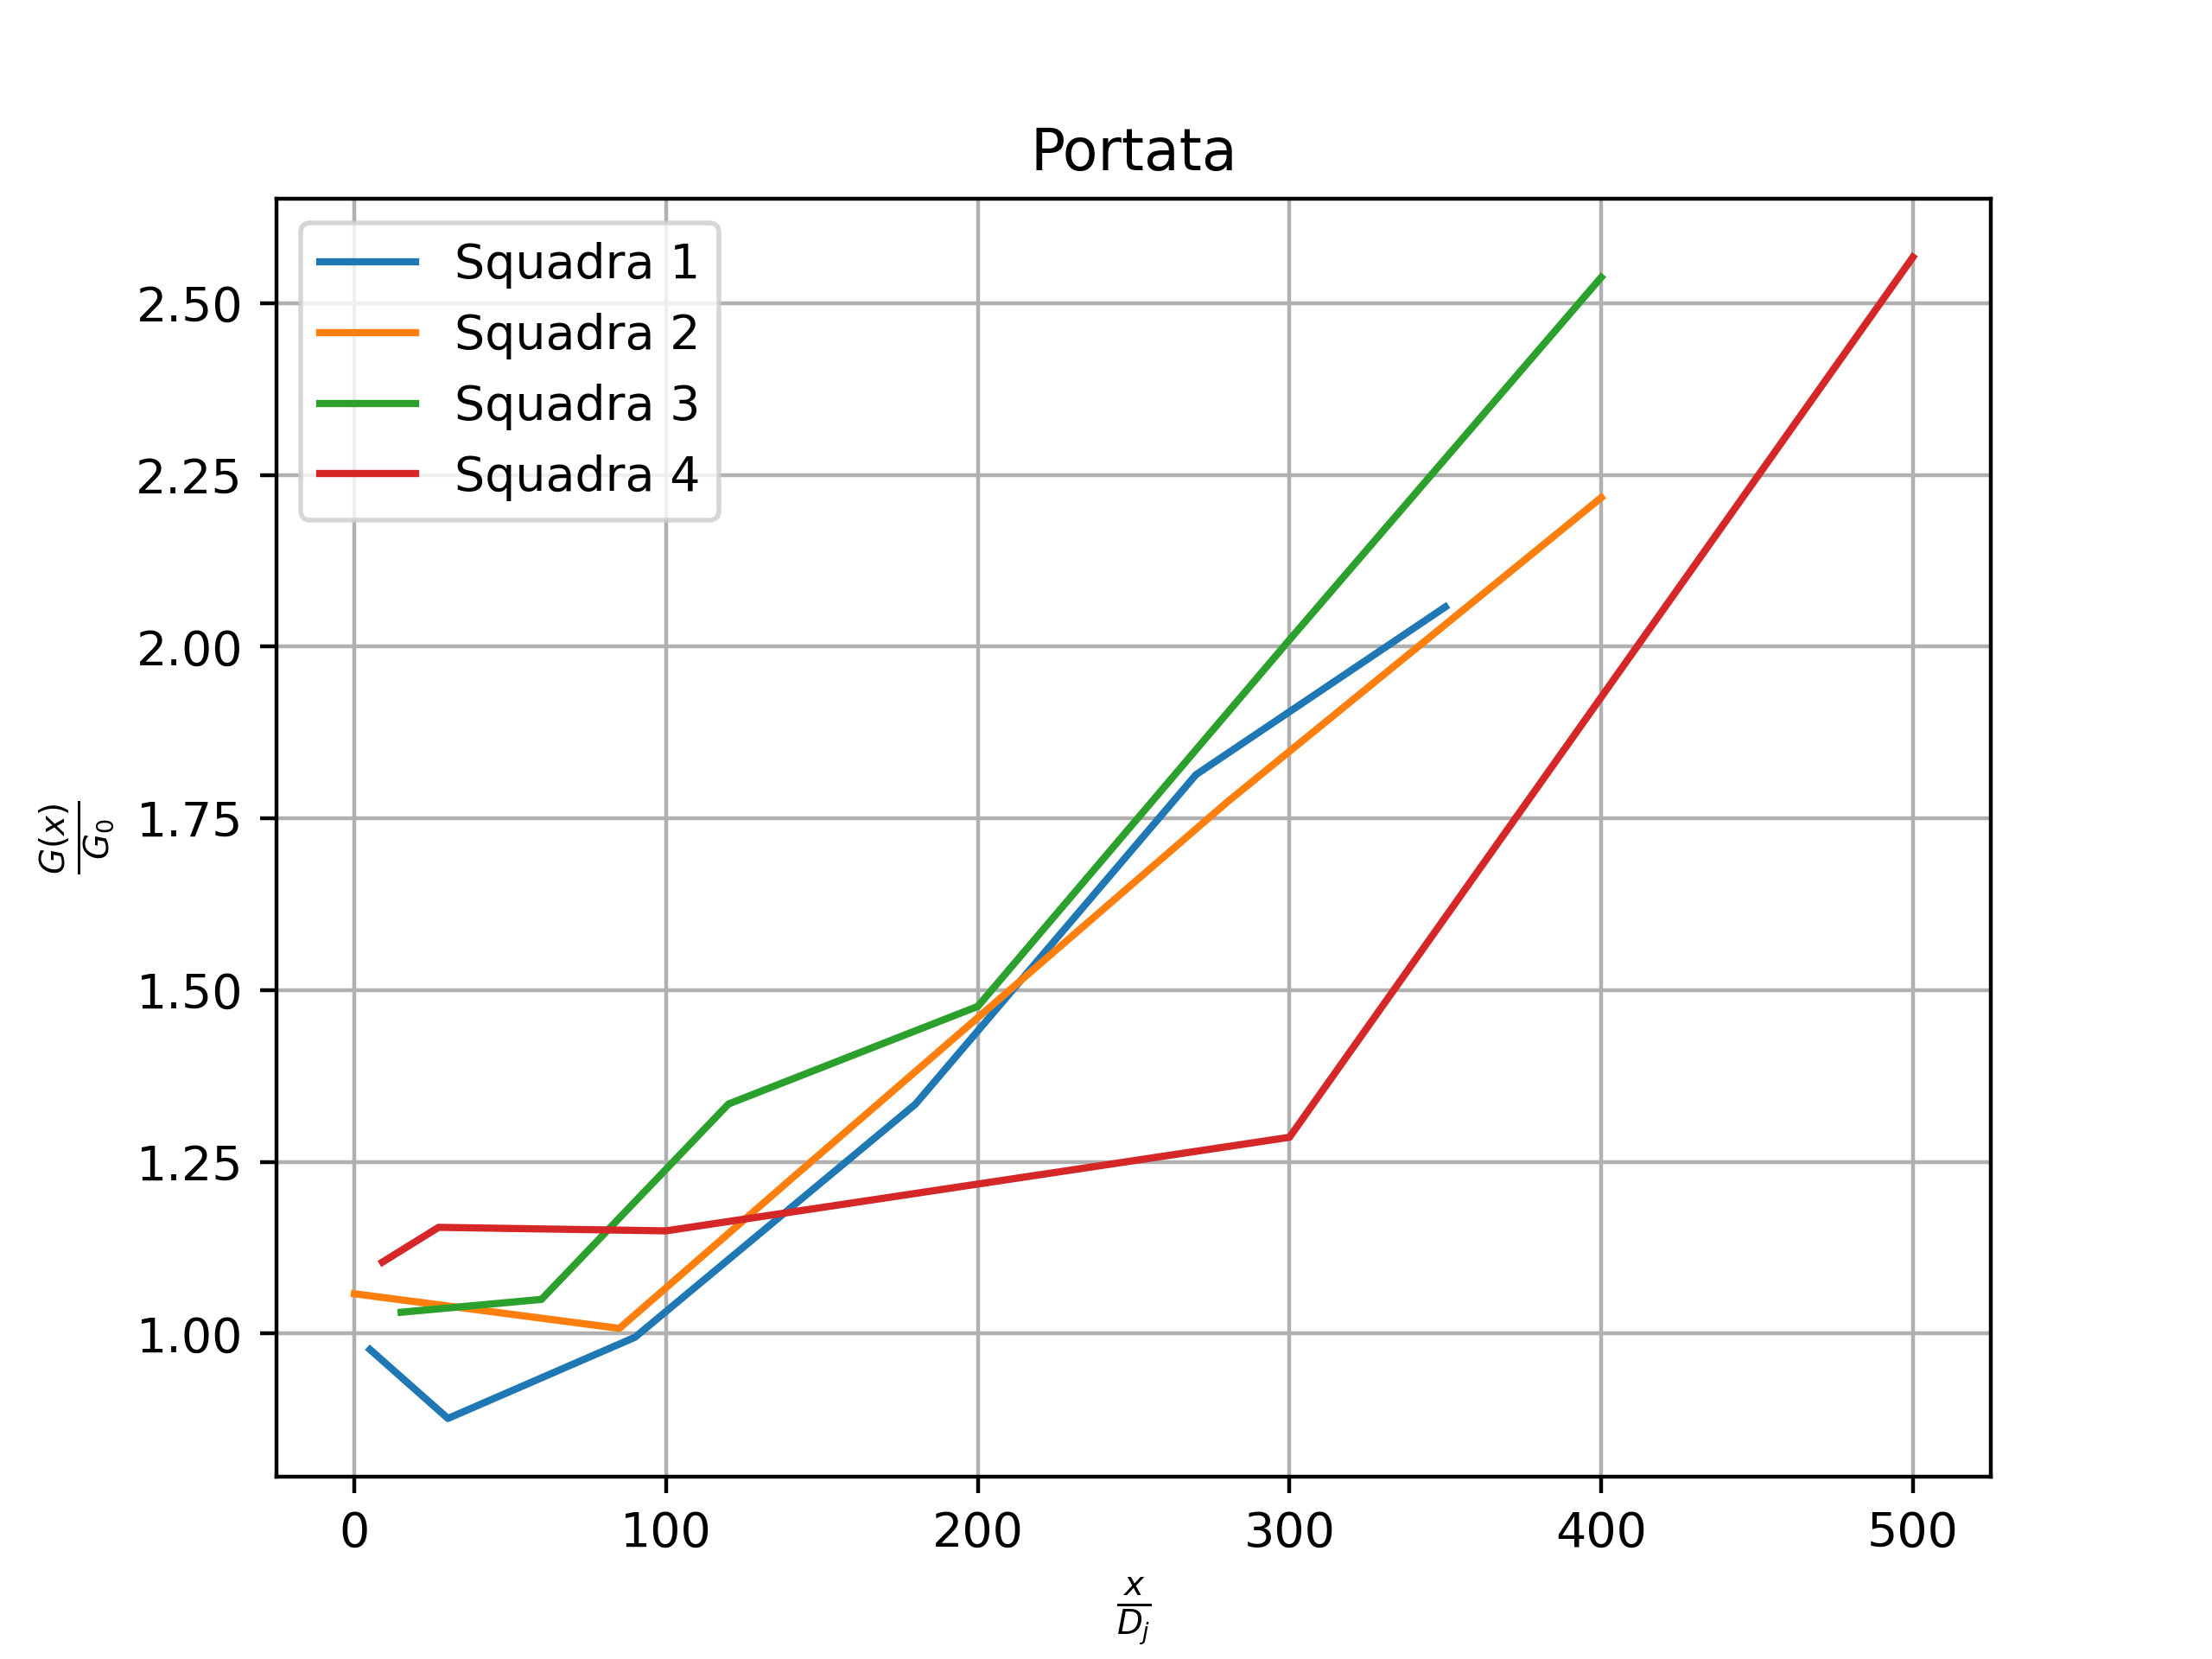
\includegraphics[width=.8\linewidth]{images/4/portata.png}
    \caption{Portata in massa}
\end{figure}

\subsection{Quantità di moto}
Poiché non sono agenti forze esterne sul flusso, è atteso che la quantità di moto lungo l'asse del getto rimanga costante.\\\\
La quantità di moto elementare è definita come:
\begin{equation*}
    dM = dG\ u = 2\pi\rho u^2 rdr
\end{equation*}
Integrando si ottiene:
\begin{equation*}
    M = 2\pi\rho \int_0^\infty u^2r dr \quad \left[\frac{kg\,m}{s^2} \right]
\end{equation*}
La quantità di moto in corrispondenza della sezione di uscita è invece:
\begin{equation*}
    M_0 = \rho \left( \frac{\pi D^2}4 \right) U_0^2
\end{equation*}
Valutando la funzione integranda in modo discreto utilizzando i dati sperimentali, è possibile risolvere l'integrale con l'applicazione della regola dei trapezi.\\\\
Diagrammando l'andamento della quantità di moto $M$, normalizzata rispetto al valore in corrispondenza della sezione di uscita $M_0$, si ottiene il seguente diagramma:
\begin{figure}[h]
    \centering
    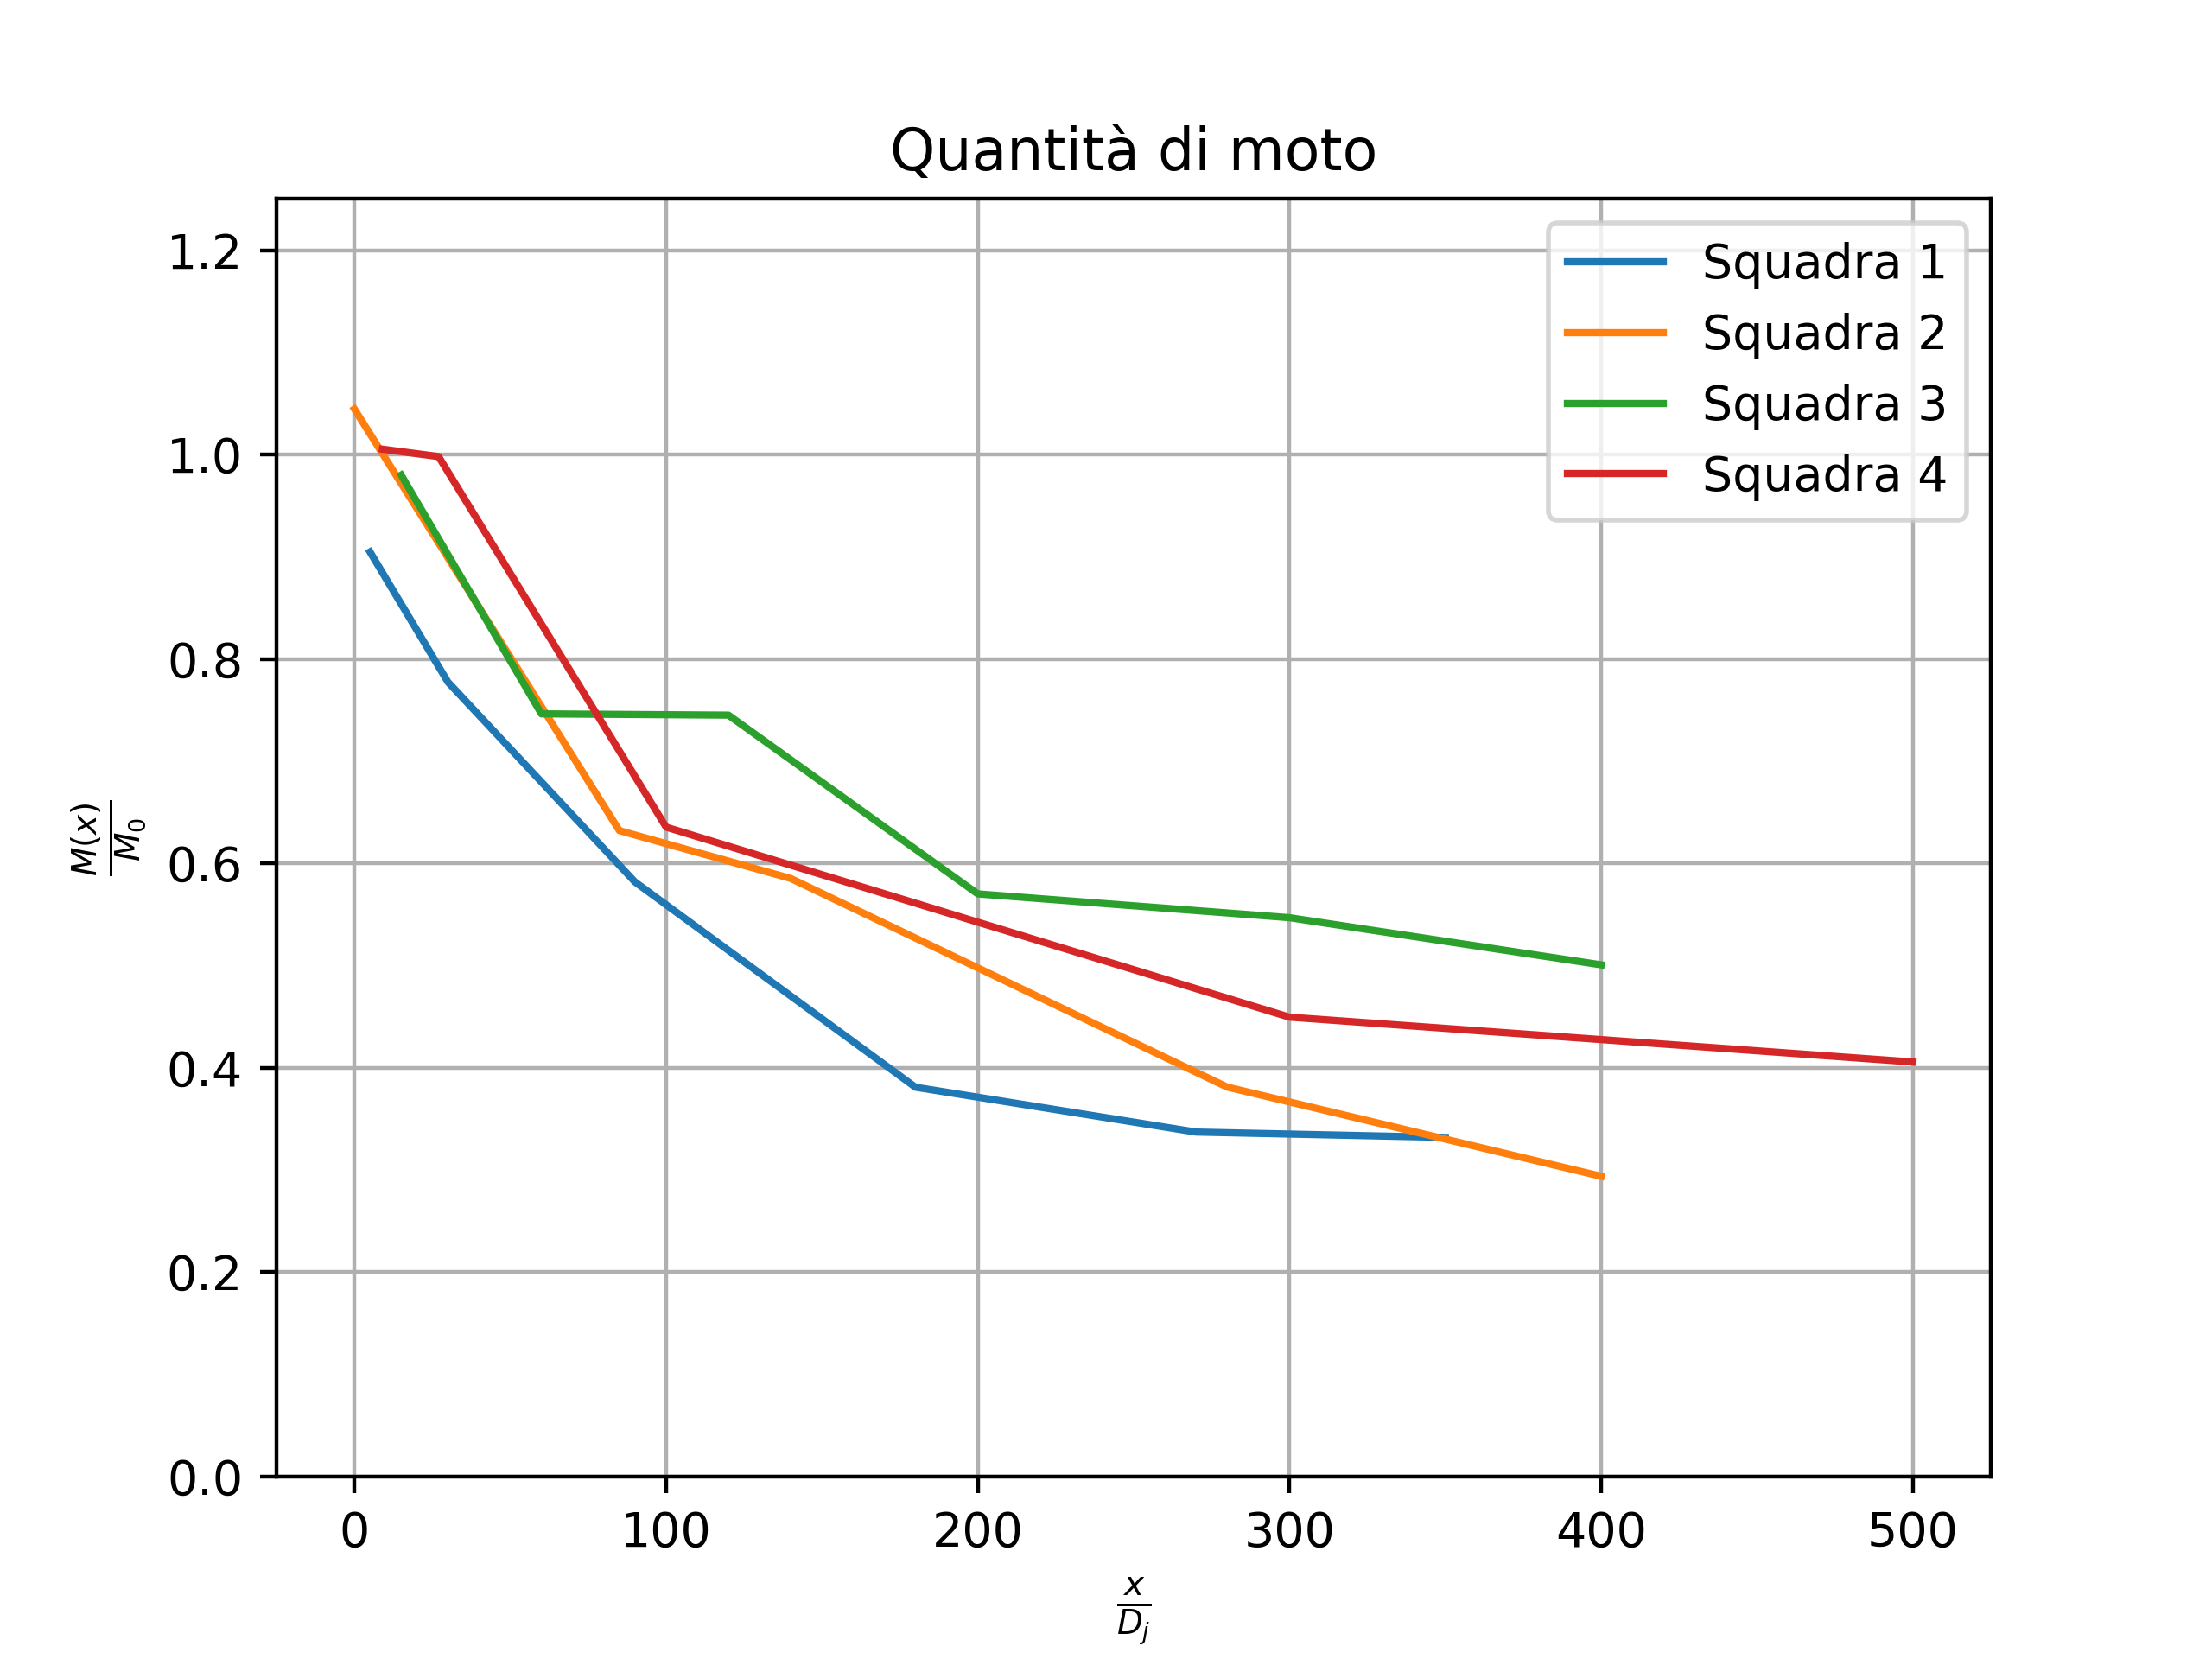
\includegraphics[width=.7\linewidth]{images/4/qdm.png}
    \caption{Quantità di moto}
\end{figure}

\noindent L'andamento decrescente è dovuto al fatto che i dati raccolti non hanno coperto una distanza radiale $r$ infinita, pertanto parte della quantità di moto non è rilevata.

\subsection{Energia}
A causa della dissipazione viscosa, l'energia si prospetta decrescente lungo l'asse del getto.\\\\
Per scrivere l'energia nell'unità di tempo che compete ad ogni sezione basta scrivere l'energia cinetica elementare del moto medio e riferirla all'unità di tempo:
\begin{equation*}
    E = \frac{dE_c}{dt} = \frac12 \frac{dm}{dt} u^2 = \frac12 G u^2 = \frac12 2\pi\rho \int_0^\infty u^3r dr
\end{equation*}
Quindi:
\begin{equation*}
    E = \pi\rho \int_0^\infty u^3r dr \quad \left[W\right]
\end{equation*}
L'energia in corrispondenza della sezione di uscita è invece:
\begin{equation*}
    E_0 = \frac12 \rho \left( \frac{\pi D^2}4 \right) U_0^3
\end{equation*}
Valutando la funzione integranda in modo discreto utilizzando i dati sperimentali, è possibile risolvere l'integrale con l'applicazione della regola dei trapezi.\\\\
Diagrammando l'andamento dell'energia $E$ normalizzata rispetto al valore in corrispondenza della sezione di uscita $E_0$ si ottiene il seguente diagramma:
\begin{figure}[h]
    \centering
    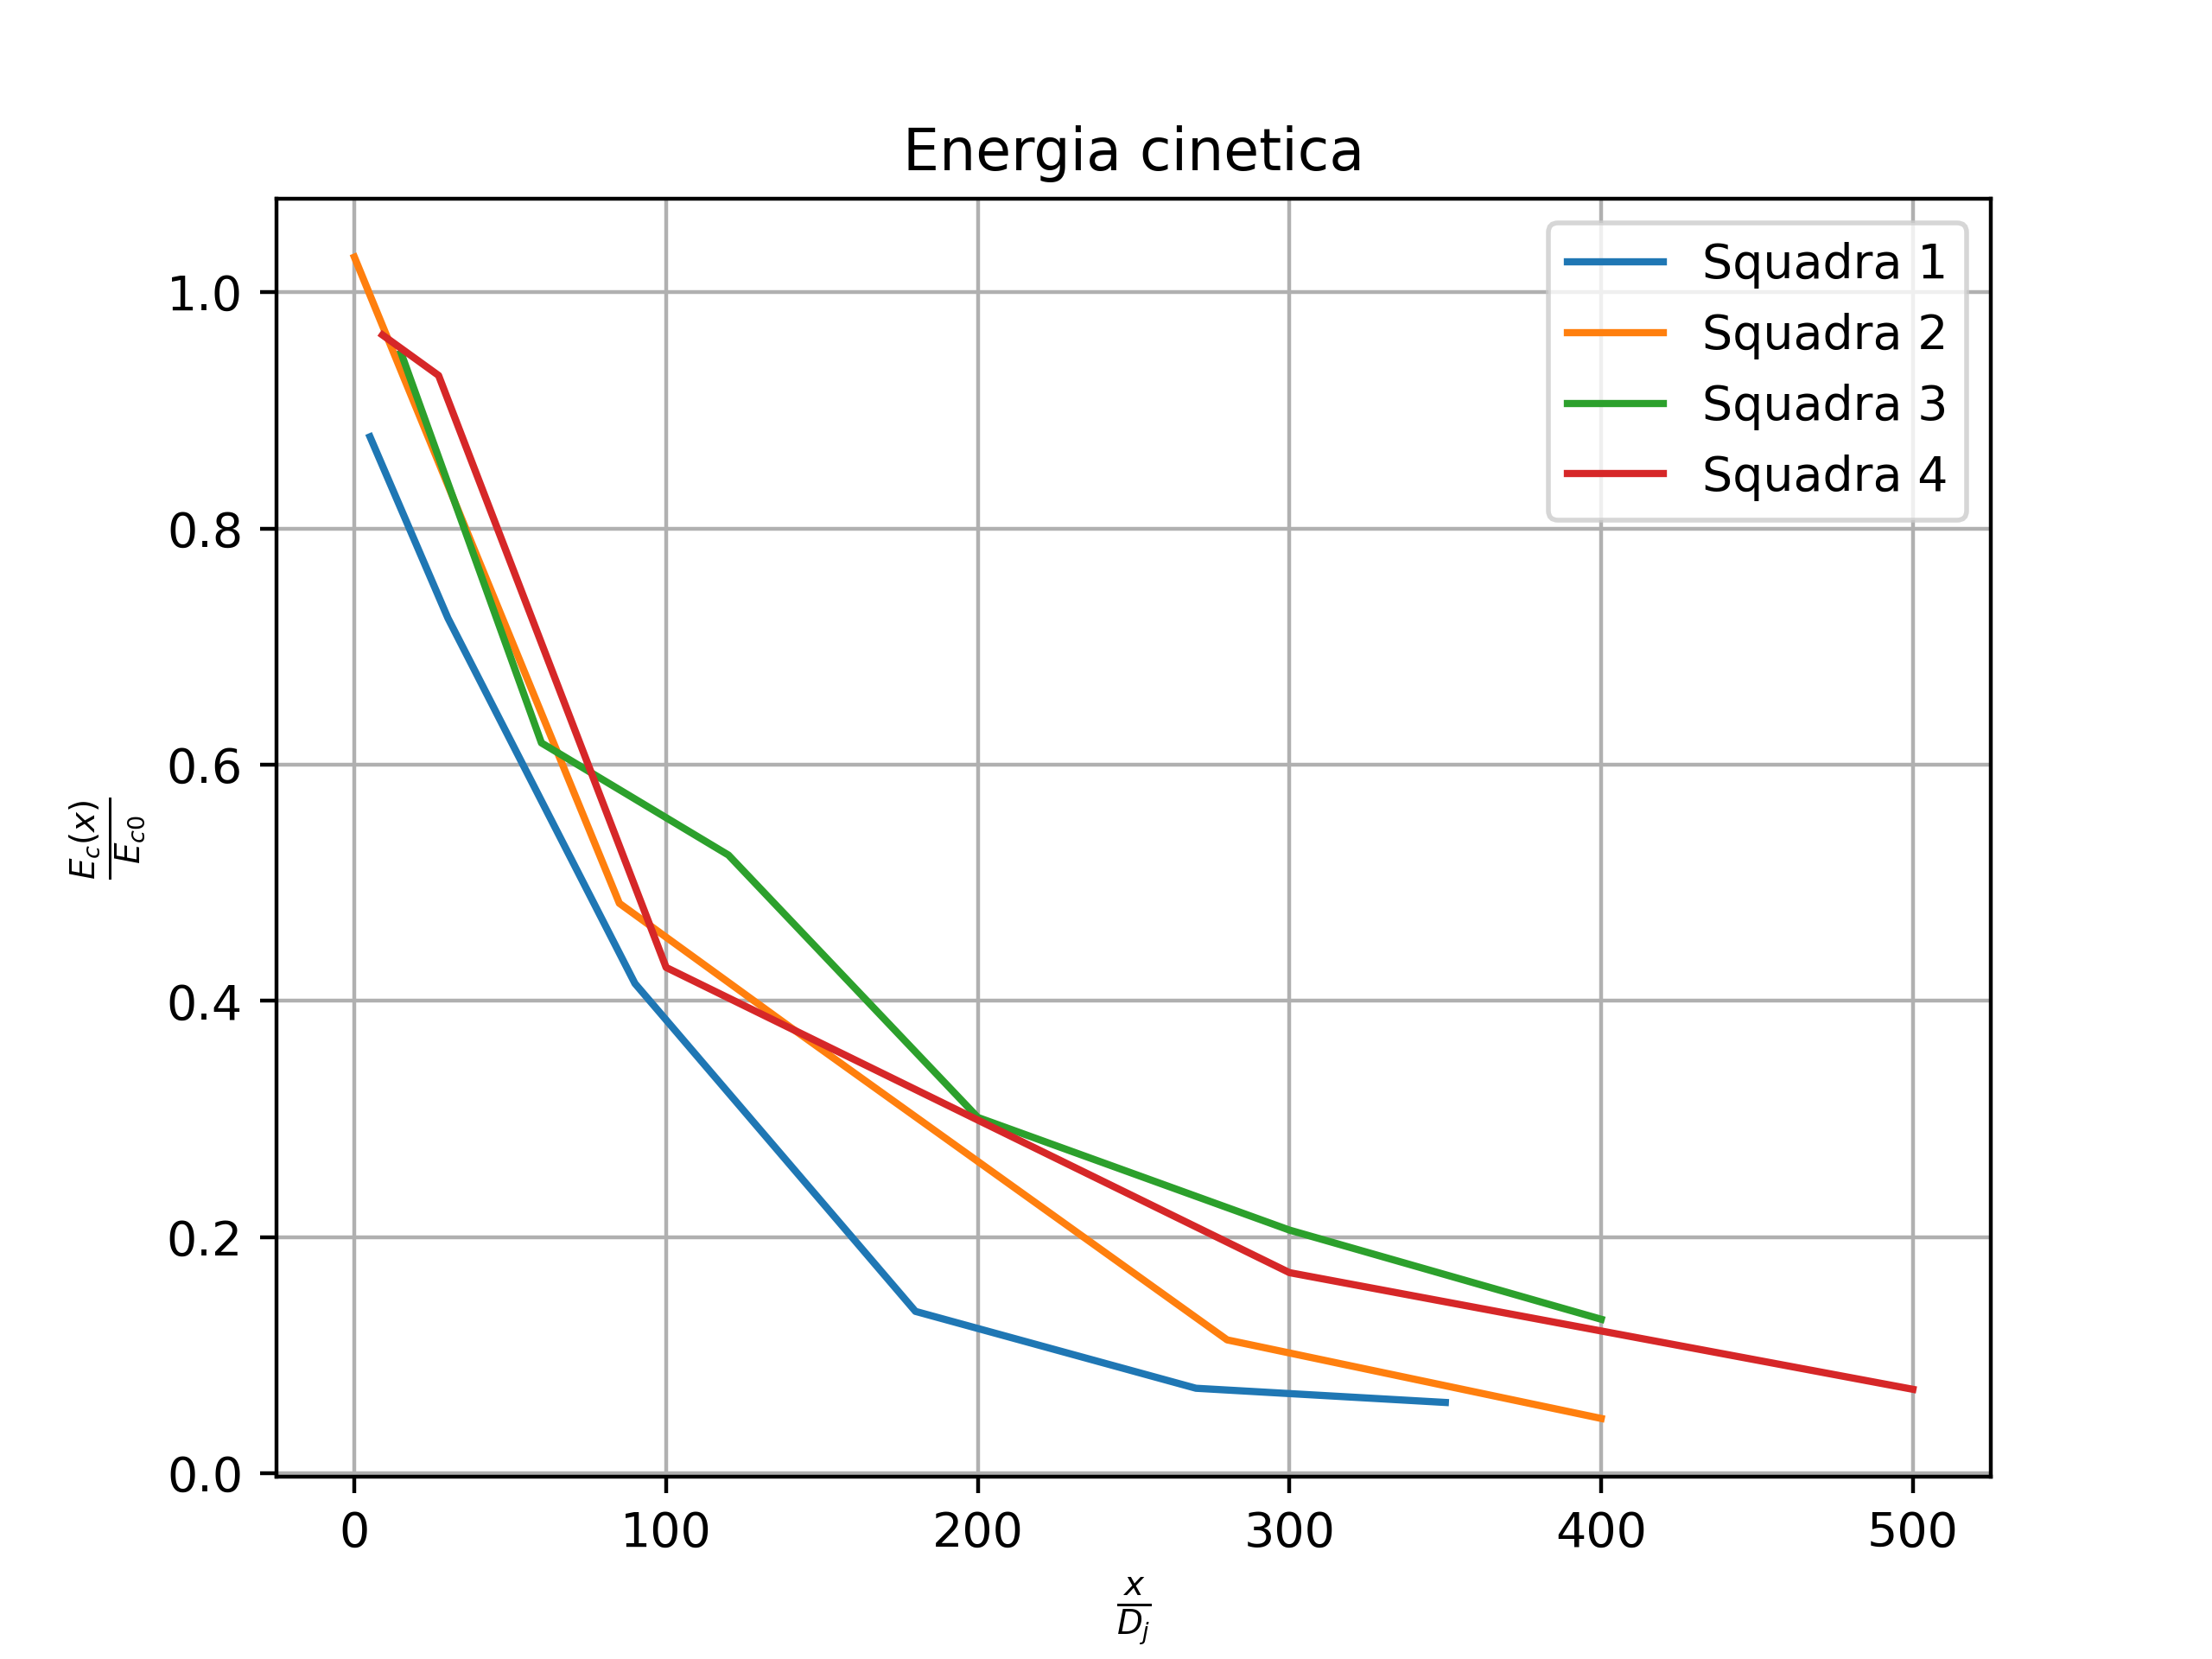
\includegraphics[width=.8\linewidth]{images/4/energia.png}
    \caption{Energia}
\end{figure}